\documentclass[10pt,a4paper]{article}
\usepackage[utf8]{inputenc}
\usepackage{graphicx}
\def\Pr{\mathop{\rm Pr}}
\usepackage[english]{babel}
\usepackage{tikz}
\usetikzlibrary{arrows,snakes,backgrounds,shapes.geometric}
\title{Probability and Statistical Inference}
\author{John S Butler}
%\date{July 2019}
\input{cheatsheet-template.tex}



%--------------------------------------------------------------------------------
\begin{document}

%\maketitle
%\thispagestyle{empty}
\scriptsize
%\tableofcontents


%\section{Data Type}
\section*{Encryption - Algorithms  (MATH1812)\footnote{\href{https://sites.google.com/dit.ie/math1812/home}{Course Website: https://sites.google.com/dit.ie/math1812/home}}}
%$\subsection*{Cheat Sheet}
\subsubsection*{\href{johnsbutler.netlify.com}{John S Butler} (TU Dublin) }

\begin{textbox}{Flowchart }
\begin{subbox}{subbox}{Caesar Cipher -Encrypt }
\begin{center}
    
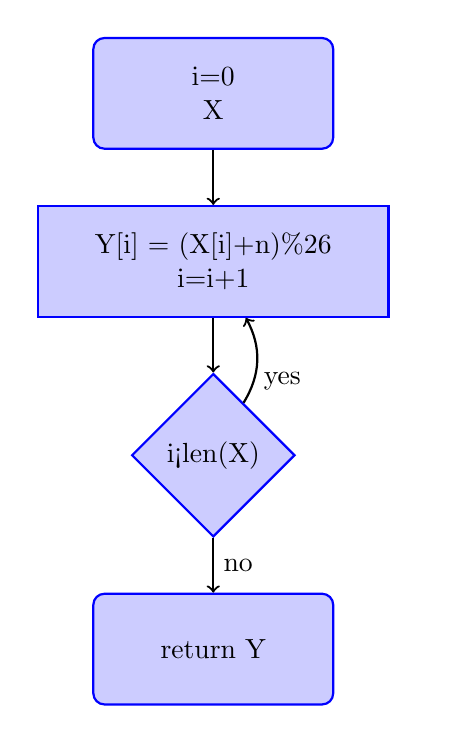
\begin{tikzpicture}[auto]
\tikzstyle{decision} = [diamond, draw=blue, thick, fill=blue!20,
text width=4.5em, text badly centered, inner sep=1pt]

\tikzstyle{block} = [rectangle, draw=blue, thick, fill=blue!20,
text width=8em, text centered, rounded corners, minimum height=4em]
\tikzstyle{block_op} = [rectangle, draw=blue, thick, fill=blue!20,
text width=12em, text centered, minimum height=4em]
\tikzstyle{line} = [draw, thick,->];
\tikzstyle{cloud} = [draw=red, thick, ellipse,fill=red!20, minimum height=2em];
\matrix [column sep=5mm,row sep=7mm]
{
%\node [cloud] (start) {X,m,c,m X}
% row 1
 \node [block] (init) {i=0 \\ X}; & \\
% row 2
\node [block_op] (identify) {Y[i] = (X[i]+n)\%26
\\
i=i+1}; & ;\\
% row 4
\node [decision] (decide) {i<len(X)}; & \\
% row 5
\node [block] (stop) {return Y}; & \\
};
\tikzstyle{every path}=[line]
\path (init) -- (identify);
\path (identify) -- (decide);
\path (decide)  edge [bend right] node[near start,right] {yes}  (identify);
\path (decide) -- node [midway] {no} (stop);

\end{tikzpicture}

\end{center}
\end{subbox}
\begin{subbox}{subbox}{Caesar Cipher -Decrypt }
\begin{center}
    
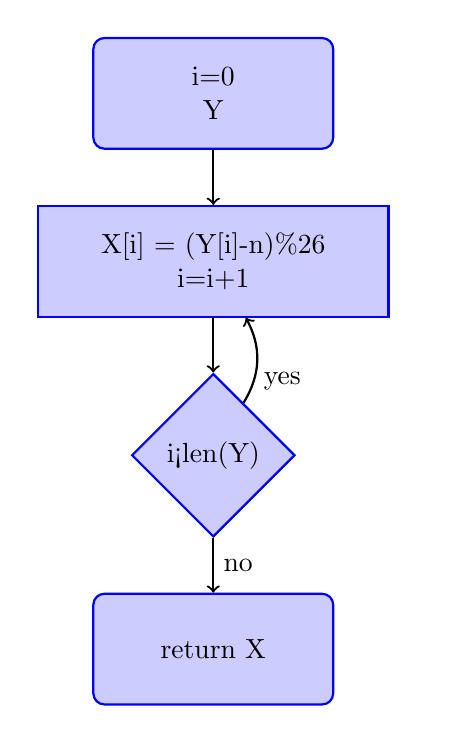
\begin{tikzpicture}[auto]
\tikzstyle{decision} = [diamond, draw=blue, thick, fill=blue!20,
text width=4.5em, text badly centered, inner sep=1pt]

\tikzstyle{block} = [rectangle, draw=blue, thick, fill=blue!20,
text width=8em, text centered, rounded corners, minimum height=4em]
\tikzstyle{block_op} = [rectangle, draw=blue, thick, fill=blue!20,
text width=12em, text centered, minimum height=4em]
\tikzstyle{line} = [draw, thick,->];
\tikzstyle{cloud} = [draw=red, thick, ellipse,fill=red!20, minimum height=2em];
\matrix [column sep=5mm,row sep=7mm]
{
%\node [cloud] (start) {X,m,c,m X}
% row 1
 \node [block] (init) {i=0 \\ Y}; & \\
% row 2
\node [block_op] (identify) {X[i] = (Y[i]-n)\%26
\\
i=i+1}; & ;\\
% row 4
\node [decision] (decide) {i<len(Y)}; & \\
% row 5
\node [block] (stop) {return X}; & \\
};
\tikzstyle{every path}=[line]
\path (init) -- (identify);
\path (identify) -- (decide);
\path (decide)  edge [bend right] node[near start,right] {yes}  (identify);
\path (decide) -- node [midway] {no} (stop);

\end{tikzpicture}

\end{center}
\end{subbox}


\end{textbox}


%%% FLOW CHART
\begin{textbox}{Psuedocode}
\begin{codebox}{r}{Caesar Cipher -Encrypt  }
def Caesar_Encrypt(X): 
# For loop from 0 to end of word X
    for i in range(0,len(X)):
        Y[i] = (X[i]+n)%26

    return Y
\end{codebox}

\begin{codebox}{r}{Caesar Cipher -Decrypt  }
def Caesar_Decrypt(Y): 
# For loop from 0 to end of word Y
    for i in range(0,len(Y)):
        X[i] = (Y[i]-n)%26

    return X
\end{codebox}
\end{textbox}
\newpage
%% Vignere
\begin{textbox}{Flowchart }
\begin{subbox}{subbox}{Vigenere Cipher -Encrypt }
\begin{center}
    
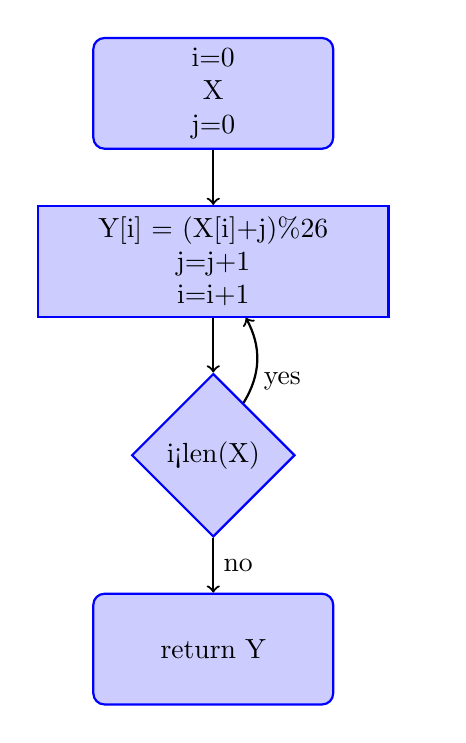
\begin{tikzpicture}[auto]
\tikzstyle{decision} = [diamond, draw=blue, thick, fill=blue!20,
text width=4.5em, text badly centered, inner sep=1pt]

\tikzstyle{block} = [rectangle, draw=blue, thick, fill=blue!20,
text width=8em, text centered, rounded corners, minimum height=4em]
\tikzstyle{block_op} = [rectangle, draw=blue, thick, fill=blue!20,
text width=12em, text centered, minimum height=4em]
\tikzstyle{line} = [draw, thick,->];
\tikzstyle{cloud} = [draw=red, thick, ellipse,fill=red!20, minimum height=2em];
\matrix [column sep=5mm,row sep=7mm]
{
%\node [cloud] (start) {X,m,c,m X}
% row 1
 \node [block] (init) {i=0 \\ X\\j=0}; & \\
% row 2
\node [block_op] (identify) {Y[i] = (X[i]+j)\%26
\\
j=j+1\\
i=i+1}; & ;\\
% row 4
\node [decision] (decide) {i<len(X)}; & \\
% row 5
\node [block] (stop) {return Y}; & \\
};
\tikzstyle{every path}=[line]
\path (init) -- (identify);
\path (identify) -- (decide);
\path (decide)  edge [bend right] node[near start,right] {yes}  (identify);
\path (decide) -- node [midway] {no} (stop);

\end{tikzpicture}

\end{center}
\end{subbox}
\begin{subbox}{subbox}{Vigenere Cipher -Decrypt }
\begin{center}
    
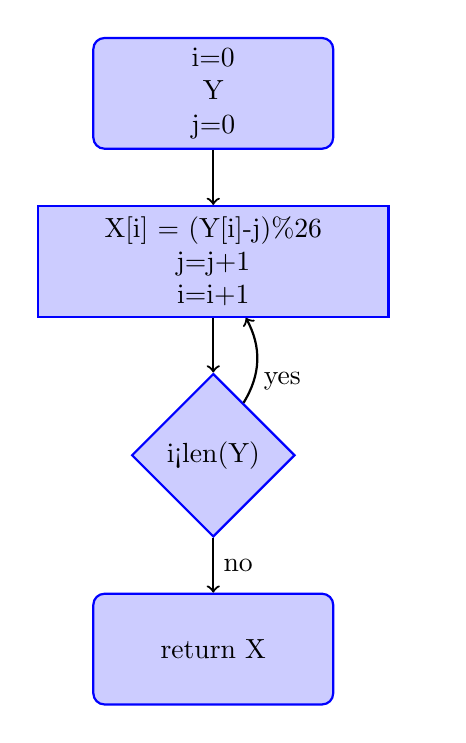
\begin{tikzpicture}[auto]
\tikzstyle{decision} = [diamond, draw=blue, thick, fill=blue!20,
text width=4.5em, text badly centered, inner sep=1pt]

\tikzstyle{block} = [rectangle, draw=blue, thick, fill=blue!20,
text width=8em, text centered, rounded corners, minimum height=4em]
\tikzstyle{block_op} = [rectangle, draw=blue, thick, fill=blue!20,
text width=12em, text centered, minimum height=4em]
\tikzstyle{line} = [draw, thick,->];
\tikzstyle{cloud} = [draw=red, thick, ellipse,fill=red!20, minimum height=2em];
\matrix [column sep=5mm,row sep=7mm]
{
%\node [cloud] (start) {X,m,c,m X}
% row 1
 \node [block] (init) {i=0 \\ Y\\j=0}; & \\
% row 2
\node [block_op] (identify) {X[i] = (Y[i]-j)\%26
\\
j=j+1\\
i=i+1}; & ;\\
% row 4
\node [decision] (decide) {i<len(Y)}; & \\
% row 5
\node [block] (stop) {return X}; & \\
};
\tikzstyle{every path}=[line]
\path (init) -- (identify);
\path (identify) -- (decide);
\path (decide)  edge [bend right] node[near start,right] {yes}  (identify);
\path (decide) -- node [midway] {no} (stop);

\end{tikzpicture}

\end{center}
\end{subbox}


\end{textbox}


%%% FLOW CHART
\begin{textbox}{Psuedocode}
\begin{codebox}{r}{Vigenere Cipher -Encrypt  }
def Vigenere_Encrypt(X): 
# For loop from 0 to end of word X
    j=0
    for i in range(0,len(X)):
        Y[i] = (X[i]+j)%26
        j=j+1

    return Y
\end{codebox}

\begin{codebox}{r}{Vigenere Cipher - Decrypt  }
def Vigenere_Decrypt(Y): 
# For loop from 0 to end of word Y
    j=0
    for i in range(0,len(Y)):
        X[i] = (Y[i]-j)%26
        j=j+1

    return X
\end{codebox}
\end{textbox}



\newpage
%% KEYWORD
%% Vignere
\begin{textbox}{Flowchart }
\begin{subbox}{subbox}{Vigenere Cipher with Keyword-Encrypt }
\begin{center}
    
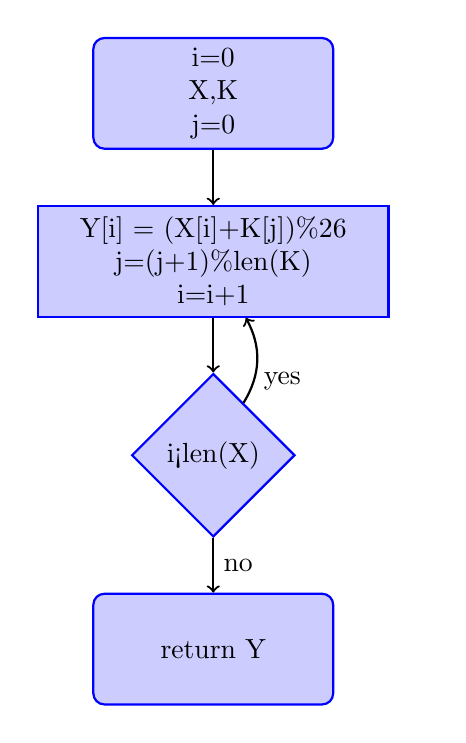
\begin{tikzpicture}[auto]
\tikzstyle{decision} = [diamond, draw=blue, thick, fill=blue!20,
text width=4.5em, text badly centered, inner sep=1pt]

\tikzstyle{block} = [rectangle, draw=blue, thick, fill=blue!20,
text width=8em, text centered, rounded corners, minimum height=4em]
\tikzstyle{block_op} = [rectangle, draw=blue, thick, fill=blue!20,
text width=12em, text centered, minimum height=4em]
\tikzstyle{line} = [draw, thick,->];
\tikzstyle{cloud} = [draw=red, thick, ellipse,fill=red!20, minimum height=2em];
\matrix [column sep=5mm,row sep=7mm]
{
%\node [cloud] (start) {X,m,c,m X}
% row 1
 \node [block] (init) {i=0 \\ X,K\\j=0}; & \\
% row 2
\node [block_op] (identify) {Y[i] = (X[i]+K[j])\%26
\\
j=(j+1)\%len(K)\\
i=i+1}; & ;\\
% row 4
\node [decision] (decide) {i<len(X)}; & \\
% row 5
\node [block] (stop) {return Y}; & \\
};
\tikzstyle{every path}=[line]
\path (init) -- (identify);
\path (identify) -- (decide);
\path (decide)  edge [bend right] node[near start,right] {yes}  (identify);
\path (decide) -- node [midway] {no} (stop);

\end{tikzpicture}

\end{center}
\end{subbox}
\begin{subbox}{subbox}{Vigenere Cipher -Decrypt }
\begin{center}
    
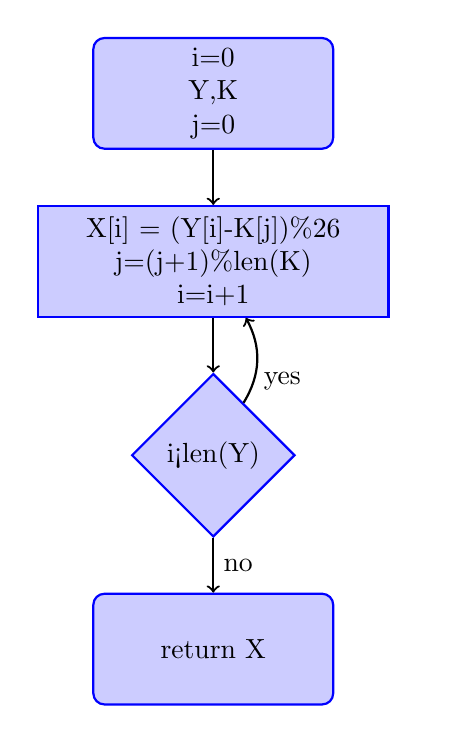
\begin{tikzpicture}[auto]
\tikzstyle{decision} = [diamond, draw=blue, thick, fill=blue!20,
text width=4.5em, text badly centered, inner sep=1pt]

\tikzstyle{block} = [rectangle, draw=blue, thick, fill=blue!20,
text width=8em, text centered, rounded corners, minimum height=4em]
\tikzstyle{block_op} = [rectangle, draw=blue, thick, fill=blue!20,
text width=12em, text centered, minimum height=4em]
\tikzstyle{line} = [draw, thick,->];
\tikzstyle{cloud} = [draw=red, thick, ellipse,fill=red!20, minimum height=2em];
\matrix [column sep=5mm,row sep=7mm]
{
%\node [cloud] (start) {X,m,c,m X}
% row 1
 \node [block] (init) {i=0 \\ Y,K\\j=0}; & \\
% row 2
\node [block_op] (identify) {X[i] = (Y[i]-K[j])\%26
\\
j=(j+1)\%len(K)\\
i=i+1}; & ;\\
% row 4
\node [decision] (decide) {i<len(Y)}; & \\
% row 5
\node [block] (stop) {return X}; & \\
};
\tikzstyle{every path}=[line]
\path (init) -- (identify);
\path (identify) -- (decide);
\path (decide)  edge [bend right] node[near start,right] {yes}  (identify);
\path (decide) -- node [midway] {no} (stop);

\end{tikzpicture}

\end{center}
\end{subbox}


\end{textbox}


%%% FLOW CHART
\begin{textbox}{Psuedocode}
\begin{codebox}{r}{Vigenere Cipher with Keyword -Encrypt  }
def Vigenere_Encrypt_with_Keyword(X,K): 
# For loop from 0 to end of word X
    j=0
    for i in range(0,len(X)):
        Y[i] = (X[i]+K[j])%26
        j=(j+1)%len(K)

    return Y
\end{codebox}

\begin{codebox}{r}{Vigenere Cipher with Keyword -Decrypt  }
def Vigenere_Decrypt_with_Keyword(Y,K): 
# For loop from 0 to end of word Y
    j=0
    for i in range(0,len(Y)):
        X[i] = (Y[i]-K[j])%26
        j=(j+1)%len(K)

    return X
\end{codebox}
\end{textbox}



\section*{Random Number - Algorithms  (MATH1812)\footnote{\href{https://sites.google.com/dit.ie/math1812/home}{Course Website: https://sites.google.com/dit.ie/math1812/home}}}
%$\subsection*{Cheat Sheet}
\subsubsection*{\href{johnsbutler.netlify.com}{John S Butler} (TU Dublin) }

\begin{textbox}{Flowchart }
\begin{subbox}{subbox}{Linear Congruential Method }
\begin{center}
    
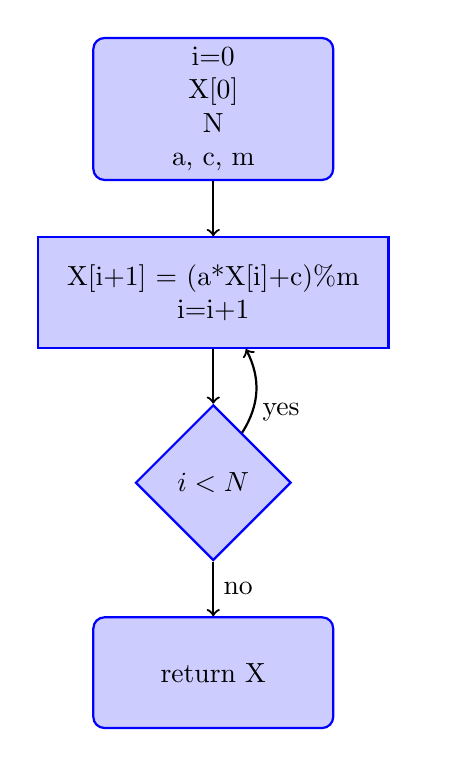
\begin{tikzpicture}[auto]
\tikzstyle{decision} = [diamond, draw=blue, thick, fill=blue!20,
text width=4.5em, text badly centered, inner sep=1pt]

\tikzstyle{block} = [rectangle, draw=blue, thick, fill=blue!20,
text width=8em, text centered, rounded corners, minimum height=4em]
\tikzstyle{block_op} = [rectangle, draw=blue, thick, fill=blue!20,
text width=12em, text centered, minimum height=4em]
\tikzstyle{line} = [draw, thick,->];
\tikzstyle{cloud} = [draw=red, thick, ellipse,fill=red!20, minimum height=2em];
\matrix [column sep=5mm,row sep=7mm]
{
%\node [cloud] (start) {X,m,c,m X}
% row 1
 \node [block] (init) {i=0 \\ X[0]\\N\\a, c, m}; & \\
% row 2
\node [block_op] (identify) {X[i+1] = (a*X[i]+c)\%m
\\
i=i+1}; & ;\\
% row 4
\node [decision] (decide) {$i<N$}; & \\
% row 5
\node [block] (stop) {return X}; & \\
};
\tikzstyle{every path}=[line]
\path (init) -- (identify);
\path (identify) -- (decide);
\path (decide)  edge [bend right] node[near start,right] {yes}  (identify);
\path (decide) -- node [midway] {no} (stop);

\end{tikzpicture}

\end{center}
\end{subbox}

\end{textbox}


%%% FLOW CHART
\begin{textbox}{Psuedocode}
\begin{codebox}{r}{Linear Congruential Method }
def Linear_Congruential_Method(a,c,m,X[0]): 
# For loop from 0 to N with steps of 1
    for i in range(0,N):
        X[i+1] = (a*X[i]+c)%m

    return X


\end{codebox}
\end{textbox}

%% Linear Congruential Method for  Numbers between A and B
\begin{textbox}{Flowchart }
\begin{subbox}{subbox}{Linear Congruential Method for  Numbers between A and B}
\begin{center}
    
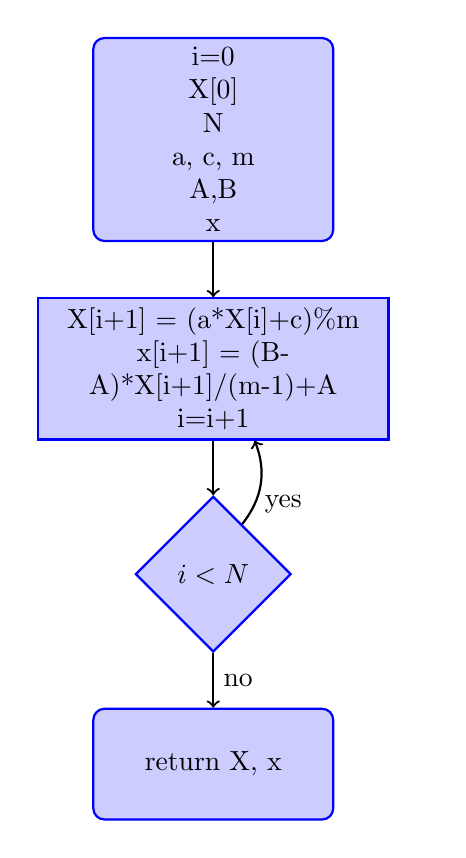
\begin{tikzpicture}[auto]
\tikzstyle{decision} = [diamond, draw=blue, thick, fill=blue!20,
text width=4.5em, text badly centered, inner sep=1pt]

\tikzstyle{block} = [rectangle, draw=blue, thick, fill=blue!20,
text width=8em, text centered, rounded corners, minimum height=4em]
\tikzstyle{block_op} = [rectangle, draw=blue, thick, fill=blue!20,
text width=12em, text centered, minimum height=4em]
\tikzstyle{line} = [draw, thick,->];
\tikzstyle{cloud} = [draw=red, thick, ellipse,fill=red!20, minimum height=2em];
\matrix [column sep=5mm,row sep=7mm]
{
%\node [cloud] (start) {X,m,c,m X}
% row 1
 \node [block] (init) {i=0 \\ X[0]\\N\\a, c, m\\ A,B\\x}; & \\
% row 2
\node [block_op] (identify) {X[i+1] = (a*X[i]+c)\%m
\\
x[i+1] = (B-A)*X[i+1]/(m-1)+A
\\
i=i+1}; & ;\\
% row 4
\node [decision] (decide) {$i<N$}; & \\
% row 5
\node [block] (stop) {return X, x}; & \\
};
\tikzstyle{every path}=[line]
\path (init) -- (identify);
\path (identify) -- (decide);
\path (decide)  edge [bend right] node[near start,right] {yes}  (identify);
\path (decide) -- node [midway] {no} (stop);

\end{tikzpicture}

\end{center}
\end{subbox}

\end{textbox}


%%% FLOW CHART
\begin{textbox}{Psuedocode}
\begin{codebox}{r}{Linear Congruential Method for  Numbers between A and B }
def Linear_Congruential_Method(a,c,m,X[0],x,A,B): 
N=len(X)
# For loop from 0 to N with steps of 1
    for i in range(0,N):
        X[i+1] = (a*X[i]+c)%m
        x[i+1]=(B-A)*X[i+1]/(m-1)+A
    return X, x


\end{codebox}
\end{textbox}
%% Linear Congruential Method for Area of a Triangle
\begin{textbox}{Flowchart }
\begin{subbox}{subbox}{Linear Congruential Method for  Numbers for Area of a Triangle}
\begin{center}
    
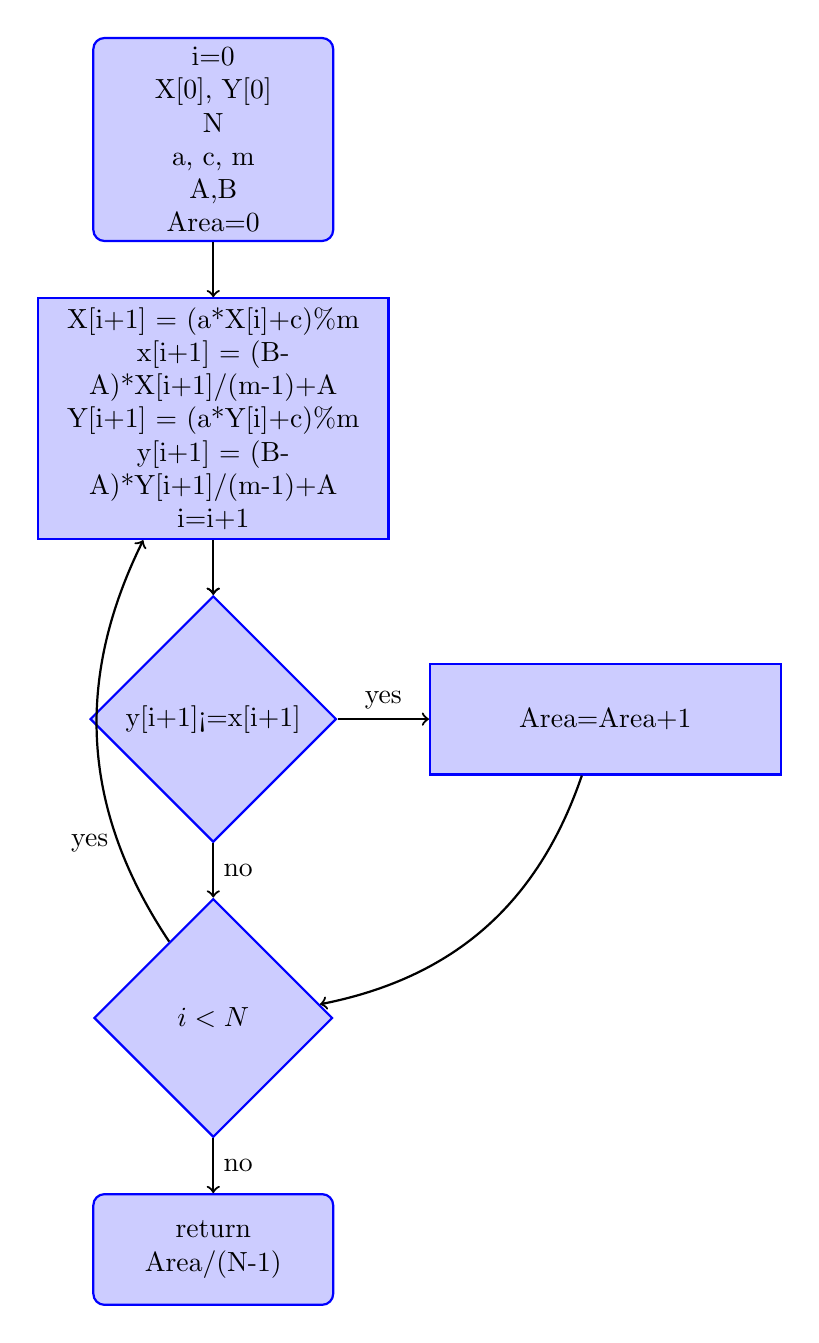
\begin{tikzpicture}[auto]
\tikzstyle{decision} = [diamond, draw=blue, thick, fill=blue!20,
text width=7.5em, text badly centered, inner sep=1pt]

\tikzstyle{block} = [rectangle, draw=blue, thick, fill=blue!20,
text width=8em, text centered, rounded corners, minimum height=4em]
\tikzstyle{block_op} = [rectangle, draw=blue, thick, fill=blue!20,
text width=12em, text centered, minimum height=4em]
\tikzstyle{line} = [draw, thick,->];
\tikzstyle{cloud} = [draw=red, thick, ellipse,fill=red!20, minimum height=2em];
\matrix [column sep=5mm,row sep=7mm]
{
%\node [cloud] (start) {X,m,c,m X}
% row 1
 \node [block] (init) {i=0 \\X[0], Y[0]\\N\\a, c, m\\ A,B\\Area=0}; & \\
% row 2
\node [block_op] (identify) {X[i+1] = (a*X[i]+c)\%m
\\
x[i+1] = (B-A)*X[i+1]/(m-1)+A\\

Y[i+1] = (a*Y[i]+c)\%m
\\
y[i+1] = (B-A)*Y[i+1]/(m-1)+A
\\
i=i+1}; & ;\\
% row 4
\node [decision] (decide_area) {y[i+1]<=x[i+1]}; & 
\node [block_op] (identify_area) {Area=Area+1}; \\

\node [decision] (decide) {$i<N$}; & \\
% row 5
\node [block] (stop) {return Area/(N-1)}; & \\
};
\tikzstyle{every path}=[line]
\path (init) -- (identify);
\path (identify) -- (decide_area);
\path (identify) -- (decide_area);
\path (decide)  edge [bend left] node[near start,left] {yes}  (identify);
\path (decide_area) -- node [midway] {no} (decide);
\path (decide_area)-- node [midway] {yes} (identify_area);
\path (identify_area)edge [bend left] (decide);
\path (decide) -- node [midway] {no} (stop);

\end{tikzpicture}

\end{center}
\end{subbox}

\end{textbox}


%%% FLOW CHART
\begin{textbox}{Psuedocode}
\begin{codebox}{r}{Linear Congruential Method for  Numbers between A and B }
def Linear_Congruential_Method(a,c,m,X[0],x,y,A,B): 
Area=0
# For loop from 0 to N with steps of 1
    for i in range(0,N):
        X[i+1] = (a*X[i]+c) % m
        
        x[i+1]=(B-A)*X[i+1]/(m-1)+A
        
        Y[i+1] = (a*Y[i]+c)% m
        
        y[i+1]=(B-A)*Y[i+1]/(m-1)+A
        if y[i+1]<=x[i+1]:
            Area=Area+1
            
    return Area/(N-1)


\end{codebox}
\end{textbox}

\end{document}
